\ProvidesFile{ch-theory.tex}

\chapter{THEORY}

\section{Circular-Restricted Three-Body Problem (CR3BP) with Control}

To model the motion of a maneuvering spacecraft in cislunar space, we utilize the circular restricted three-body problem dynamics model with low-thrust control modeled as an affine acceleration. This model assumes circular motion of two massive primary bodies around their barycenter. A third massless body is then subject to the gravities of the other two massive bodies. This third body represents the spacecraft of interest, and its state $\bm{\xi} = [\bm{r}^\top, \bm{v}^\top]^\top$ consists of a three-dimensional position and velocity, $\bm{r} = [x, y, z]^\top$ and $\bm{v} = [v_x, v_y, v_z]^\top$, respectively. The control is a three-dimensional additive acceleration $\bm{u} = [u_x, u_y, u_z]^\top$. To define the coordinate frame, the origin is fixed at the barycenter, the X-axis is aligned with the line between the two massive bodies, the Z-axis is aligned with the angular velocity vector, and the Y-axis completes the X-Y-Z right-handed coordinate frame. The CR3BP coordinate frame is illustrated in Figure \ref{fig:CR3BP}. 

The units of the system are normalized such that the unit length is the distance between the two massive bodies, and the unit time is the inverse of the angular velocity of the two massive bodies. The motion of the massless body is then described by a system of nonlinear differential equations given by 
\begin{align}
\begin{aligned}
    \dot{\bm{\xi}} &= \bm{g}(\bm{\xi}) + B\bm{u}= \begin{bmatrix}
        v_x \\
        v_y \\
        v_z \\
        -\frac{(1 - \mu)(x + \mu)}{d^2} - \frac{\mu(x + \mu - 1)}{r^2} + 2v_y + x\\
        -\frac{(1 - \mu)y}{d^2} - \frac{\mu y}{r^2} - 2v_x + y\\
        -\frac{(1 - \mu)z}{d^2} - \frac{\mu z}{r^2}
    \end{bmatrix} + \begin{bmatrix}
        0_{3 \times 3} \\
        I_3
    \end{bmatrix} \begin{bmatrix}
        u_x \\
        u_y \\
        u_z
    \end{bmatrix} \\
    d &= \sqrt{(x+\mu)^2 + y^2 + z^2}, \quad r = \sqrt{(x + \mu - 1)^2 + y^2 + z^2} \label{eq:CR3BP-dynamics}
\end{aligned}
\end{align}
\noindent where $\mu = m_2/(m_1 + m_2)$ is the ratio of the second body's mass to the total mass of the system \cite{zimovan2017characteristics}.

\section{Periodic Orbits in the CR3BP}

% \begin{figure}
%     \centering
%     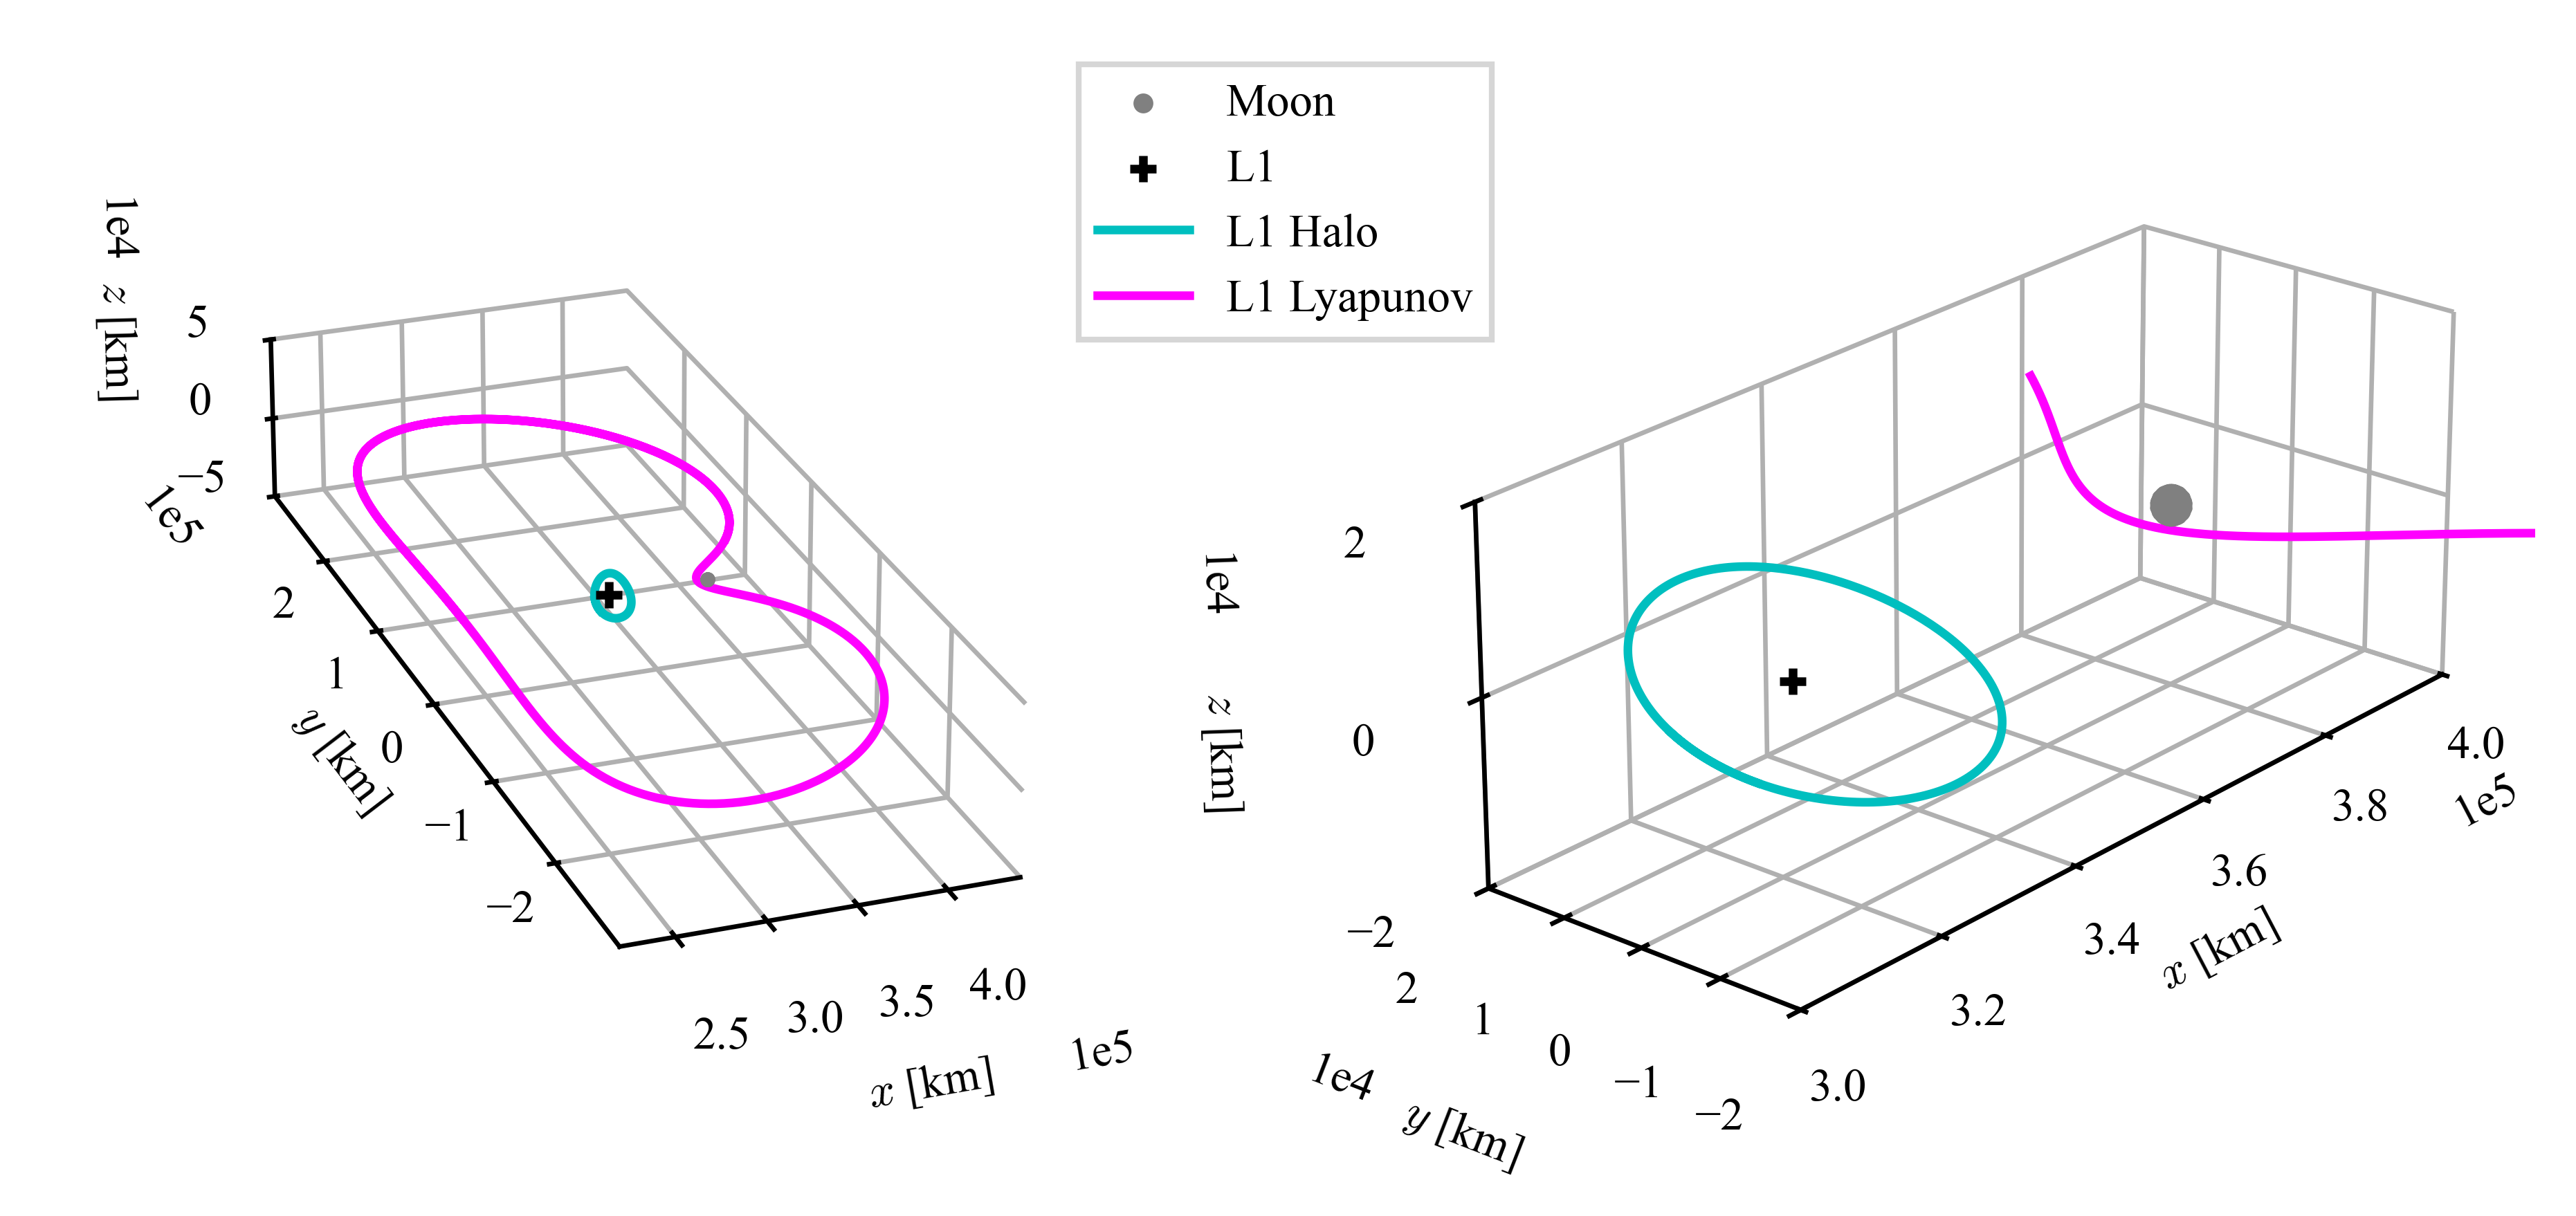
\includegraphics[width=0.85\linewidth]{Figures/orbits.png}
%     \caption{Representative L1 Lyapunov and L1 Halo Periodic Orbits}
%     \label{fig:orbits}
% \end{figure}

It is desirable to obtain periodic solutions $\bm{\gamma}$ to the CR3BP dynamics (Eq. \ref{eq:CR3BP-dynamics}), such that
\begin{align}
    \bm{\gamma}(t + T) = \bm{\gamma}(t)
\end{align}
\noindent where $T$ is the period of the solution. These periodic orbits enable geometries impossible when only considering a single body's gravity. However, the dynamics of the CR3BP (Eq. \ref{eq:CR3BP-dynamics}) have no analytical closed-form solution, so these orbits are typically obtained using numerical methods.

Once a periodic solution has been obtained, continuation strategies can be employed to obtain a family of similar solutions \cite{williams2024dynamics}. The orbits of interest in this paper are those belonging to the L1 Lyapunov and L1 Halo families. These families are associated with the L1 Lagrange point, with the L1 Lyapunov family lying in the xy-plane and the L1 Halo family being three dimensional. These solutions are unstable, increasing the difficulty of the tracking problem, as small estimation errors caused by perturbations or maneuvers quickly expand during periods without observations. The representative orbits of interest are plotted in Figure \ref{fig:orbits}.

\section{Extended Kalman Filter (EKF)}

The ubiquitous Extended Kalman Filter (EKF) is an recursive estimation algorithm for systems with nonlinear dynamics/measurements \cite{smith1962application}. One iteration of the continuous-discrete EKF consists of two steps: a continuous time update and a discrete measurement update.

\begin{enumerate}
    \item Time Update
    
    The time update propagates the posterior estimate ${}^+\hat{\bm{x}}_{k-1}$ and estimation error covariance ${}^+P_{k-1}$ at the time of the previous measurement $t_{k-1}$ to the time of the current measurement $t_k$. The state is propagated with the nonlinear dynamics equation $\dot{\bm{x}} = \bm{f}(\bm{x})$, and the covariance is propagated with the state transition matrix $\Phi(t_k, t_{k-1})$ and process noise covariance $Q_{k-1}$, yielding the prior estimate and covariance at the current time, ${}^-\bm{\hat{x}}_k$ and ${}^-P_k$:
    \begin{align}
        {}^-\hat{\bm{x}}_k &= \int_{t_{k-1}}^{t_k} \bm{f}(\bm{\hat{x}}(t)) dt, & \hat{\bm{x}}(t_{k-1}) = {}^+\hat{\bm{x}}_{k-1} \label{nonlinear estimate propagation (first EKF equation)} \\
        {}^-P_k &= \Phi(t_k, t_{k-1}) {}^+P_{k-1} \Phi^\top(t_k, t_{k-1}) + Q_{k-1}\\
        \Phi(t_k, t_{k-1}) &= \int_{t_{k-1}}^{t_k} F(\hat{\bm{x}}(\tau))\Phi(\tau, t_{k-1}) d\tau, & \Phi(t_{k-1}, t_{k-1}) = I_{n\times n} \label{eq:STM-propagation}
    \end{align}
    Additionally, the nonlinear measurement equation $\bm{z} = \bm{h}(\bm{x})$ is applied to the prior estimate ${}^-\hat{\bm{x}}_k$ to obtain the predicted measurement, $\bm{\hat{z}}_k$.
    \begin{align}
        \bm{\hat{z}}_k = \bm{h}_k(\bm{\hat{x}}_k^-) \label{eq:predicted measurement}
    \end{align}

    \item Measurement Update
    
    After the time update, ${}^-\bm{\hat{x}}_k$ and ${}^-P_k$ are updated with the new measurement $\bm{z}_k = \bm{h}_k(\bm{x}_k) + \bm{w}_k$ to obtain the posterior estimate and covariance, ${}^-\bm{x}_k$ and ${}^+P_k$. Mathematically,
    \begin{align}
        ^+\bm{\hat{x}}_k &= K_k (\bm{z}_k - \bm{\hat{z}}_k) \label{eq:posterior-estimate-update}\\
        ^+P_k &= {}^-P_k - C_k K_k^\top - K_k C_k ^\top + K_k W_k K_k^\top \\
        K_k &= C_k W_k^{-1} \\
        C_k &= {}^-P_k H_k^\top({}^-\bm{\hat{x}}_k) \\
        W_k &= H_k({}^-\bm{\hat{x}}_k) {}^-P_k H_k^\top({}^-\bm{\hat{x}}_k) + R_k \label{eq:innovations covariance (last EKF eq)}
    \end{align}
    \noindent where $K_k$ is the Kalman gain matrix, $C_k$ is the cross covariance matrix, $W_k$ is the innovations covariance matrix, $H_k({}^-\bm{\hat{x}}_k) = \partial \bm{h}({}^-\hat{\bm{x}}_k)/\partial\bm{x}$ is the measurement Jacobian, and $R_k = \mathcal{E}[\bm{w}_k\bm{w}_k^\top]$ is the measurement noise covariance.

\end{enumerate}

At the completion of the measurement update, one iteration of the EKF is completed, and the next iteration begins after setting $ t_k \rightarrow t_{k-1}$. 

\section{Interacting Multiple Model (IMM) Estimator}

The interacting multiple model (IMM) estimator is well-suited for tracking maneuvering targets because of its ability to incorporate multiple dynamics models into a single filter \cite{blom1988interacting,bar1989tracking,genovese2001interacting}. These different dynamics models can capture the discrete ``modes" of a maneuvering target which yields a more accurate estimate. 

Mathematically, the IMM assumes that the target's mode $\tau_k$ at time $t_k$ is one of $s$ discrete modes in the set of all modes $M = \{1, \cdots, s\}$, such that $\tau_k \in M $. Each mode $j \in M$ is associated with a dynamics model $\dot{\bm{x}} = \bm{f}^{(j)}(\bm{x})$, process noise covariance $Q^{(j)}$, posterior state estimate ${}^+\hat{\bm{x}}_k^{(j)}$, posterior estimate error covariance ${}^+P_k^{(j)}$, and mode probability $\mu^{(j)}_k = \mathbb{P}\{\tau_k = j\}$. The time evolution of these modes are modeled as a discrete-time Markov chain with associated row-stochastic transition matrix $\Pi \in \mathbb{R}^{s \times s}$, where element $\Pi_{i, j} = \mathbb{P}\{\tau_k=j \mid \tau_{k-1} = i\}$.

One iteration of the IMM consists of three steps: probabilistic mixing, mode-dependent filtering, and mode probability update.

\begin{enumerate}
    \item Probabilistic Mixing

    The posterior state estimates ${}^+\hat{\bm{x}}_{k-1}^{(j)}$ and covariances ${}^+P_{k-1}^{(j)}$ are probabilistically combined to create mode-matched initial conditions for the mode-dependent filtering in the following step. The mode-matched estimate and covariance for each mode $j$ is denoted as ${}^{+}\hat{\bm{x}}_{k-1}^{0j}$ and ${}^+P_{k-1}^{0j}$, respectively, and are obtained with
    \begin{align}
        {}^+\hat{\bm{x}}_{k-1}^{0j} &= \sum_{i=1}^r {}^+\hat{\bm{x}}_{k-1}^{(i)} \mu_{k-1}^{i \mid j} \label{eq:mixed-initial-mean}\\
        {}^+P_{k-1}^{0j} &= \sum_{i=1}^r  \mu_{k-1}^{i \mid j} [{}^+P_{k-1}^{(i)} + ({}^+\bm{\hat{x}}_{k-1}^{(i)} - {}^+\bm{\hat{x}}_{k-1}^{0j})({}^+\bm{\hat{x}}_{k-1}^{(i)} - {}^+\bm{\hat{x}}_{k-1}^{0j})^\top ] \label{eq:mixed-initial-covariance}
    \end{align}
    \noindent where $\mu_k^{i \mid j}$ is the mixing probability, which captures how much of mode $i$'s posterior estimate should be mixed into mode $j$'s initial conditions. The mixing probabilities $\mu_k^{i \mid j}$ are computed as
    \begin{align}
        \mu_{k-1}^{i \mid j} &= \frac{1}{\bar{c}_{k-1}^{(j)}} \Pi_{i,j} \mu_{k-1}^{(i)} \\
        \bar{c}_{k-1}^{(j)} &= \sum_{i=1}^r \Pi_{i,j} \mu_{k-1}^{(i)} \label{mixing probability constant}
    \end{align}
    \noindent where $\bar{c}_{k-1}^{(j)}$ is a normalization constant such that $\sum_{i=1}^r \mu_{k-1}^{i \mid j} = 1$.
    
    \item Mode-Dependent Filtering

    After constructing the mode-matched initial conditions, an iteration of the EKF is performed for each mode $j \in M$ with Eqs. \ref{nonlinear estimate propagation (first EKF equation)}-\ref{eq:innovations covariance (last EKF eq)}, each with its own mode-matched initial conditions ${}^+\bm{\hat{x}}_{k-1}^{0j}$ and ${}^+P_{k-1}^{0j}$, dynamics equation $\bm{f}^{(j)}(\bm{x})$, and process noise covariance $Q^{(j)}$. This yields the posterior estimates and covariances for each mode ${}^+\hat{\bm{x}}_k^{(j)}$ and ${}^+P_k^{(j)}$.

    \item Mode Probability Update

    In addition to obtaining ${}^+\hat{\bm{x}}_k^{(j)}$ and ${}^+P_k^{(j)}$, the mode probabilities are updated according to the innovations likelihoods $\Lambda_k^{(j)}$ given by
    \begin{align}
        \Lambda_k^{(j)} = \dfrac{1}{\sqrt{\mid 2\pi W_k^{(j)} \mid}} \exp[-\frac{1}{2} (\bm{z}_k - \bm{\hat{z}}_k^{(j)})^\top (W_k^{(j)})^{-1} (\bm{z}_k - \bm{\hat{z}}_k^{(j)})] \label{eq:innovations-likelihoods}
    \end{align}
    where $W_k^{(j)}$ is mode $j$'s innovations covariance defined in Eq. \ref{eq:innovations covariance (last EKF eq)}, and $\hat{\bm{z}}_k^{(j)}$ is mode $j$'s predicted measurement defined in Eq. \ref{eq:predicted measurement}. The mode probability update is 
    \begin{align}
    \mu_k^{(j)} & = \frac{1}{c_k} \Lambda_k^{(j)} \bar{c}_{k-1}^{(j)} \label{eq:mode-probability-update} \\
    c_k &= \sum_{i=1}^r \Lambda_k^{(i)} \bar{c}_{k-1}^{(i)} 
    \end{align}
    where $\bar{c}_{k-1}^{(j)}$ is defined in Eq. \ref{mixing probability constant} and $c_k$ is a normalization constant such that $\sum_{j=1}^r \mu_k^{(j)} = 1$. The computation of the mode probabilities concludes a single iteration of the IMM, and the next iteration begins after setting $t_k \rightarrow t_{k-1}$.

    \item Output

    To obtain a single output value for the posterior estimate ${}^+\hat{\bm{x}}_k$ and posterior covariance ${}^+P_k $, the various posterior estimates ${}^+\hat{\bm{x}}_k^{(j)}$ and covariances ${}^+P_k^{(j)}$ are combined using their mode probabilities $\mu_k^{(j)}$:
    \begin{align}
        {}^+\bm{\hat{x}}_k &= \sum_{j=1}^r \mu_k^{(j)} {}^+\bm{\hat{x}}_k^{(j)}  \\
        {}^+P_k &= \sum_{j=1}^r \mu_k^j [{}^+P_k^{(j)} + ({}^+\bm{\hat{x}}_k^{(j)} - {}^+\bm{\hat{x}}_k)({}^+\bm{\hat{x}}_k^{(j)} - {}^+\bm{\hat{x}}_k)^\top]
    \end{align}
    Note that computing these values is not necessary to iterate the IMM and is purely for output purposes.
    
\end{enumerate}


\section{Pontryagin's Minimum Principle}

A generic optimal control problem can be defined as
\begin{align}
\begin{split}
     \min_{\bm{x}(t), \bm{u}(t)} & \quad J = \int_{t_0}^{t_f} L(t, \bm{x}(t), \bm{u}(t)) dt \\
     \text{s.t.} & \quad  \dot{\bm{x}} = \bm{f}(t, \bm{x}, \bm{u}) \\
     & \quad \bm{\psi}(\bm{x}_0, \bm{x}_f, t_0, t_f) = \bm{0}
\end{split}
\end{align}
\noindent where $J$ is the cost to be minimized, $L$ is the Lagrangian cost, $\bm{f}$ is the dynamics equation, and $\bm{\psi}$ is the vector of boundary conditions. To obtain the conditions for optimality, we utilize Pontryagin's Minimum Principle (PMP), which states that the optimal control $\bm{u}^*(t)$ is given by
\begin{align}
    \bm{u}^*(t) = \argmin_{\bm{u}(t)} H(t, \bm{x}^*(t), \bm{u}(t), \bm{\lambda}(t)) \label{PMP optimal control}
\end{align}
\noindent where $H$ is the control Hamiltonian, defined as
\begin{align}
    H(t, \bm{x}(t), \bm{u}(t), \bm{\lambda}(t)) = L + \bm{\lambda}^\top \bm{f}(\bm{x}, \bm{u}) \label{PMP Hamiltonian}
\end{align}
\noindent and $\bm{\lambda} \in \mathbb{R}^{\text{dim}(\bm{x})}$ is the costate \cite{pontryagin1962}. The costate is governed by its own dynamics, given by
\begin{equation}
    \dot{\bm{\lambda}} = -\left(\frac{\partial H}{\partial\bm{x}} \right)^\top \label{PMP costate dynamics}
\end{equation}
Using PMP, optimality can be defined mathematically as a system of dynamical equations with the augmented state $\bm{x} = [\bm{\xi}^\top, \bm{\lambda}^\top]^\top$ for use in a sequential filtering algorithm, such as the IMM.
